\documentclass{acm_proc_article-sp}

\usepackage{graphicx}

% Metadata Information


%\category{F.1.1}{Models of Computation}{Self-modifying machines (e.g., neural networks)}
%\category{I.3.3}{Computer Graphics}{Picture/Image Generation}

% Document starts
\begin{document}

% Page heads
\markboth{Owen Mooney}{Using Neural Networks to Generate Artistic Images}

% Title portion
\title{Using Neural Networks to Generate Artistic Images}
\author{Owen Mooney}

\maketitle

\begin{abstract}
Artificial Neural Networks are computational tools that have found widespread use in a number of varied fields in computer science. In particular they have had widespread success in many areas of computer graphics, for example in image classification \cite{Zhang:1992:ANN:503720.503776}, face detection \cite{Lee:2002:EAF:646864.708276} and recognition \cite{Zhao:2003:FRL:954339.954342}, and image restoration \cite{deCastro:2008:RIM:1363686.1364088}. Neural Networks are particularly efficient for these tasks since they are well suited for recognising and classifying patterns in input data. This paper investigates how it might be possible to generate aesthetically pleasing images using a Neural Network with random input data. The Neural Network could be trained by using either a fitness function or through human interaction, and thus could learn how to construct an image that would be visually appealing.
\end{abstract}

\section{Introduction}
\label{sec:intro}
An Artificial Neural Network is a system of independent processing units arranged in layers and with each unit being connected to all others in the layers above and below it. Each unit has multiple inputs and outputs, with the outputs from the previous layer being the inputs to the next, thus the structure of the network forms a directed acyclic graph. This structure is known as a \textit{Feed Forward Neural Network}. It is also possible to create a \textit{Recurrent Neural Network}, i.e. one where the graph will contain cycles, however these types of networks will not be discussed in this paper. The structure of a basic Neural Network is shown in figure \ref{fig:nnimg}. This network has an input and output layer and one \textit{hidden} layer. The number of hidden layers can be varied depending on the specific problem the network aims to solve.
\begin{figure}[h]
\textit{\caption{A graphical representation of the structure of a Neural Network}}
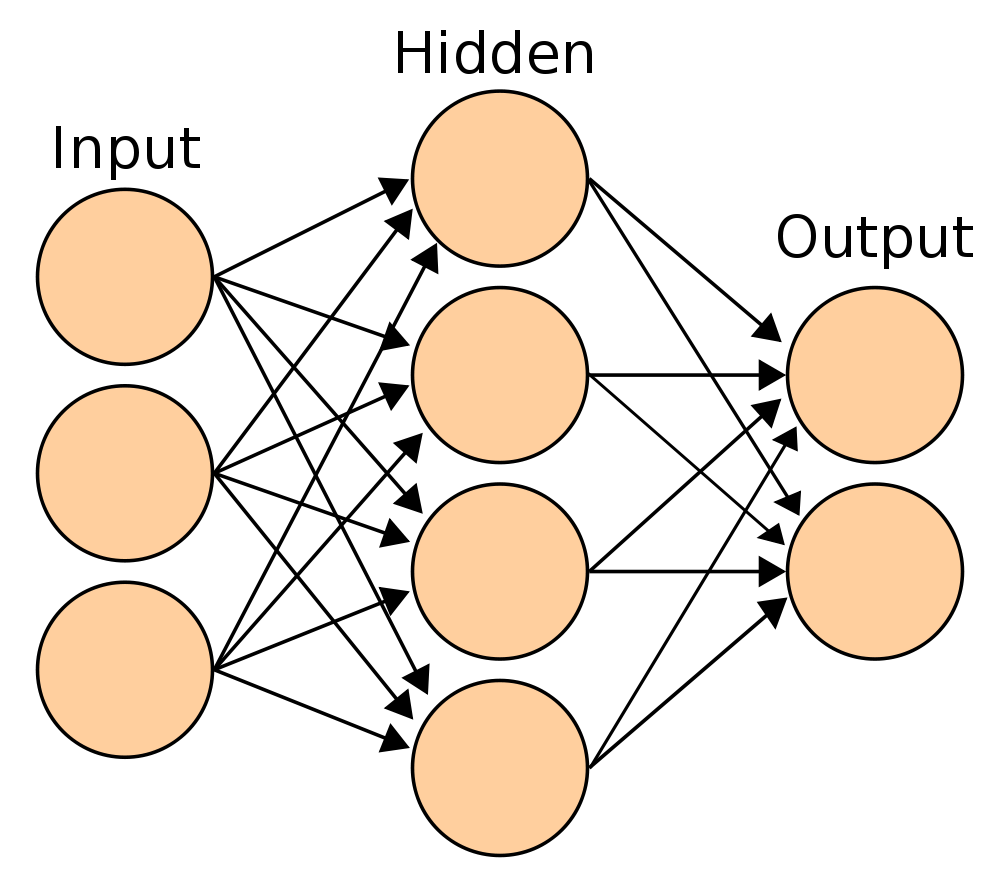
\includegraphics[width=83mm]{neuralnet1000.png}
\label{fig:nnimg}
\end{figure} 

\vspace{3mm}

In designing a Neural Network, there are a number of choices to be made. The first is the choice of combination function. This function determines how the inputs for each unit are combined to produce a \textit{net input} for the unit. Most Neural Networks use either a linear combination of the inputs, or a Euclidean distance function. Feed Forward Neural Networks are broken down into two main types depending on the function they use. These are the \textit{Multi-layer Perceptron (MLP)} in the case of the linear combination function, and the \textit{Radial Basis Function (RBF)} in the case of the Euclidean distance function. In this paper, only MLP networks will be discussed. The net input, $\nu_{k}$, for each unit is calculated as follows

\begin{equation}
\nu_{k} = \sum\limits_{j = 1}^{n} w_{k j} x_{j}
\label{eqn:one}
\end{equation}

where $w_{k j}$ is the weight associated with the connection from unit $j$ in the previous layer, $x_{j}$ is the output from the $j$-th unit in the previous layer, and $n$ is the total number of units in the previous layer. 

\vspace{3mm}

The second design choice that must be made is the activation function. This function determines how the net input, as calculated above, is converted into the output value for the unit. In many Neural Network implementations, including the one discussed in this paper, before the net input is transformed by the activation function, it is reduced by an amount know as the \textit{threshold} for the unit. It will be shown in \textit{Section \ref{sec:method}} that this value can be altered as part of the learning process for the network. Denoting the threshold for the $k$-th unit as $\tau_{k}$, the output for that unit$\sigma_{k}$ will be given by

\begin{equation}
\sigma_{k} = \phi(\nu_{k} - \tau_{k})
\end{equation}

where $\phi$ is the activation function. The activation function should be one that exhibits non-linearity, since a multi-layered network with a linear activation function can be reduced to a single layer network, thus losing the full computational power of a MLP. Two common activation functions are the hyperbolic tangent function, and the logistic function

\begin{equation}
\label{eqn:logistic}
\phi(x) = \frac{1}{1 + e^{-x}}
\end{equation}

\vspace{3mm}

A further design choice to be considered, is how the network will learn. Typically the network will learn by adjusting the weights of the connections and the threshold values for each unit. The changes that need to be made to the network can be computed by the difference between the output of the network given a certain input, and the desired output. \textit{Back Propagation} is the technique that is typically used to achieve this \cite{bertsekas1995nonlinear}.The details of its operation are beyond the scope of this paper, since it is not the learning technique used in this project. Other possibilities for learning algorithms are using genetic or evolutionary techniques, these will be discussed further in the following section.

\section{Method Outline}
\label{sec:method}

As explained above, the Neural Network used for this project is a feed-forward multi-layer perceptron, using simple linear combination as the combination function. The activation function used is the logistic function defined in equation (\ref{eqn:logistic}). The inputs to the network will be a set of real numbers between zero and one and will be randomly generated. The random input data should act as a 'seed' for the image generation. The idea behind this is that the network should be able to generate different images for different input, but that each image generated should fulfil the criteria for being an aesthetically pleasing image. Thus the network will be a general algorithm for generating visually appealing images. The possible uses of such an algorithm are discussed in \textit{Section \ref{sec:appl}}. 

\vspace{3mm} 

In a network of this type, the learning process consists of altering the connection weights and threshold values of each unit, in such a way that the output performs better as measured by some criteria. Thus these values encode the 'knowledge' of the network. Using back propagation as a training method requires that the desired output be exactly known from a given input. In this case the desired output, (that of a visually appealing image), is too poorly defined to use this technique. Thus an evolutionary algorithm is used to train the network. Every iteration of the application produces a number of distinct images, which are computed by a corresponding number of different variations of the network. The best image (as defined by the user or a fitness function) is chosen, and that network is used as the base for the next iteration. The learning rate of the network can be changed by altering the number of variations to the network structure generated in each iteration.

\vspace{3mm}

The outputs from the network are a set of real numbers between one and zero. Each image is generated using a number of coloured primitives, whose dimensions, position and colour are defined by the outputs from the network. The best image can be chosen by the user, or by calculating some metric for each image. Possible metrics to be used to determine what constitutes a good image are: colour distribution, primitive size, coverage of image space and distance between primitives. 

\section{Implementation}
\label{sec:impl}
The application accompanying this paper is written in C++, and uses OpenGL and GLUT for rendering. The network has eight inputs, four hidden layers that consist of eighty units, and eighty outputs. The image is generated from a number of coloured rectangles. Each of these takes eight parameters: x and y coordinates, height, width, and an RGBA colour value. In the current implementation the alpha value has no effect on the rendering. Since there are eighty outputs from the network, each image consists of ten rectangles. As described before, each iteration of the program produces eight different variations of the network, and an image for each one of these is generated. To reduce the memory cost of storing eight different networks, only one network is stored in full in memory. For each variation, a number of different changes to the weights and thresholds are generated. After these changes are applied, they can be reverted. This allows one network to generate eight distinct images using eight different variations. Once the best variation is chosen, the changes that produced that variation are applied permanently to the network and the cycle begins again. The structure of the network can be written to and read from disk, allowing its state to persist after the program exits.

\vspace{3mm}

The program can operate in two distinct ways. In one, the user can select the most pleasing image out of the eight using the mouse, and thus pick the best variation of the network. The other mode allows a fitness function to be evaluated for each image, and the best image chosen by the application itself. When using the fitness function, there are four parameters that affect how the different criteria are weighted, one for each of the different criteria by which the images are judged. The criteria are the colour brightness, the average distance between the rectangles, the fraction of the total image space that are covered by rectangles, and the difference between the average area of the rectangles and a target area value. These values can be changed at runtime.

\vspace{3mm}

Each unit in the network is an instance of a \textbf{Perceptron} object. These objects expose the following functionality:

\begin{verbatim}
class Perceptron
{
public:
    virtual void Increment(float amount);
    virtual float GetValue();
    virtual void Reset();
    float threshold;
protected:
    float currentValue;	
};
\end{verbatim}

The \textbf{Increment} function applies the inputs to the unit, and the current net input value is stored in the field \textbf{currentValue}. The function \textbf{GetValue} applies the activation function to the net input and returns the result. The \textbf{Reset} function simply resets the net input counter to zero. The input and output units are subclasses of this and are named \textbf{InputNode} and \textbf{OutputNode} respectively, as shown below:

\begin{verbatim}
class InputNode : public Perceptron
{
public:
    void SetValue(float amount);
};

class OutputNode : public Perceptron
{
public:
    float GetValue();
};
\end{verbatim}

The \textbf{SetValue} function allows the value of the \textbf{InputNode} to be set directly, and the \textbf{GetValue} function allows the normalised output from each \textbf{OutputNode} to be read.

\vspace{3mm}

Each connection in the network is an instance of a \textbf{Connection} object:

\begin{verbatim}
class Connection
{
public:
    Connection(int index, float weight, 
        Perceptron* endPoint, int outIndex);
    void Activate(float amount);
    int inputIndex;
    float weight;
    int outputIndex;
private:
    Perceptron* connected;
};
\end{verbatim}

The constructor takes four parameters, the array index of the input unit, the weight of the connection, a pointer to the \textbf{Perceptron} object that it is connected to, and that units array index. The \textbf{Activate} function takes the output value from the input unit and calls the \textbf{Increment} function on the unit it is connected to with that value as its argument. The \textbf{weight} field simply stores the connection weight. The \textbf{inputIndex} and \textbf{outputIndex} fields are necessary for serialisation of the class when the network is saved to a file.

\vspace{3mm}

Each layer of the network is implemented as an array of \textbf{Perceptron} objects, and an array of \textbf{Connection} objects. To compute the output of the network, first the input layer is initialised with the input data using the \textbf{SetValue} function as outlined above. Then each successive layer first computes the outputs from each unit, and the \textbf{Activate} method is called on each \textbf{Connection} object with the output from each unit as its argument. Finally the outputs are collected from the \textbf{OutputNode} objects. These outputs are used to create rectangles that are drawn to the screen. 

\section{Results}
\label{sec:results}



\section{Further Enhancements}
\label{sec:enhance}

\section{Possible Applications}
\label{sec:appl}
\bibliographystyle{abbrv}
\bibliography{report}

\end{document}